\documentclass{article}

% Font
\usepackage[T1]{fontenc}
\usepackage[utf8]{inputenc}
\usepackage{lmodern}

% For tables
\usepackage{multirow}

% For identing the table at the right place
\usepackage{float}

% For left spacing
\usepackage{scrextend}

% For images
\usepackage{graphicx}

% for shorter paragraph spaces
\setlength{\parindent}{1ex}
\setlength{\parskip}{0.5ex}
% for first paragraphs
\newcommand*\fpar{\hspace{1ex}}

\title{Project 1 Requirements}
\author{Group 14 \\
Tiago Carvalho fc51034 \\
Diogo Lopes fc51058 \\
João Roque fc51080 \\
Miguel Saldanha fc51072 \\
João Afonso fc51111 \\
}
\date{21/04/2021}

\begin{document}
\maketitle

\section{Use Cases}
  \begin{table}[H]
    \centering
    \begin{tabular}{c|c|l} 
      Services & Role & Functionalities                 \\ \hline
      \multirow{11}{*}{ Normal }
        & \multirow{5}{*}{ Any } 
          & User Log in                                 \\
        & & User Sign in                                \\
        & & Search for username                         \\
        & & See Book, Show and Movie Library            \\ 
        & & Get top 10 Items with more likes            \\ \cline{2-3}
        & \multirow{4}{*}{ User } 
          & Set Book/Show/Movie as seen/unseen          \\
        & & Set Book/Show/Movie as liked/disliked       \\ 
        & & Ask for suggestions to read and/or watch    \\ 
        & & Delete account                              \\ \cline{2-3}
      & \multirow{2}{*}{ Admin } 
          & Add Book/Show/Movie to Library              \\
        & & Remove Book/Show/Movie from Library         \\ \hline
      \multirow{2}{*}{ Spark }
        & \multirow{2}{*}{ Any }
          & See best Director in terms of rating*       \\
        & & See which worker has the most connections   \\
    \end{tabular}
    \caption{Seen's Use cases                           \\
            \**at least with $10$ movies and $10.000$ reviews in each}
  \end{table}

\section{Preliminary Functional and Non-Functional Requirements}
\fpar \textbf{SPARK note}: For the first Spark request we use a complex SQL query, for the second request we use a graph approach, which fix very nicely to the Spark capabilities.
  
  \subsection{Functional}
    \begin{itemize}
      \item Any person should be able to sign/log in with a new account.
      \item Any person should be able to search for a username
      \item Any person should be able to browse Books, Shows and Movies.
      \item Any person should be able to search for a specific item by name, type and/or categories.
      \item Any person should be able to the get the top ten liked items
      \item User should be able to mark an Item as seen/unseen.
      \item User should be able to mark an Item as liked/unliked.
      \item User should be able to ask for suggestions.
      \item Admin should be able to add and remove content from the library.
      \item \textbf{(Spark)} User should be able to see who's the best director and the worker with most connection with other workers.
    \end{itemize}

  \subsection{Non-Functional}
    \begin{itemize}
      \item Browsing Items shouldn't take more than $1.5$ seconds to load.
      \item Searching shouldn't take more than $1.5$ seconds loading the response.
      \item Marking Item as seen or liked shouldn't take loading time on Users' end.
      \item Suggestions shouldn't take more than $5$ seconds.
      \item Data stored in cache shouldn't affect the system.
      \item Adding and Removing Items should persist on the database.
      \item \textbf{Spark} request should not return error.
      \item \textbf{Spark} should and take less than $10$ minutes.
    \end{itemize}

\section{Preliminary Architectural Design}
  \begin{figure}[H]
    \centering
    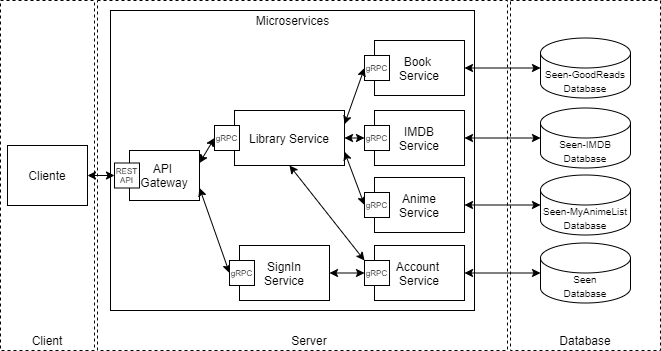
\includegraphics[width=\textwidth]{"images/CloudNativeAppArchitecture.png"}
  \end{figure}

\end{document}